\documentclass[aspectratio=169,11pt]{beamer}
\usetheme{Madrid}
\usecolortheme{seahorse}
\usefonttheme{professionalfonts}
\usepackage{amsmath,amssymb,bm,booktabs,array,graphicx,hyperref}
\usepackage{tikz}
\usetikzlibrary{positioning,arrows.meta,shapes.geometric,calc}
\usepackage{listings,xcolor,xeCJK,fontspec}
\graphicspath{{../outputs/}}
\setmainfont{texgyreheros-regular.otf}[BoldFont=texgyreheros-bold.otf,ItalicFont=texgyreheros-italic.otf]
\setsansfont{texgyreheros-regular.otf}[BoldFont=texgyreheros-bold.otf,ItalicFont=texgyreheros-italic.otf]
\setmonofont{lmmono10-regular.otf}[BoldFont=lmmonolt10-bold.otf]
\setCJKmainfont{FandolHei-Regular.otf}
\setCJKsansfont{FandolHei-Regular.otf}
\setCJKmonofont{FandolFang-Regular.otf}
\definecolor{myblue}{RGB}{36,88,135}
\definecolor{mygreen}{RGB}{40,120,80}
\definecolor{mygray}{RGB}{90,90,90}
\definecolor{myorange}{RGB}{180,100,30}
\setbeamercolor{title}{fg=myblue}
\setbeamercolor{frametitle}{fg=myblue}
\setbeamercolor{structure}{fg=myblue}
\setbeamercolor{block title}{bg=myblue,fg=white}
\setbeamercolor{block body}{bg=blue!5,fg=black}
\setbeamercolor{alertblock title}{bg=myorange,fg=white}
\setbeamercolor{alertblock body}{bg=orange!8,fg=black}
\setbeamertemplate{navigation symbols}{}
\setbeamertemplate{footline}[frame number]
\lstset{basicstyle=\ttfamily\scriptsize,keywordstyle=\color{myblue}\bfseries,stringstyle=\color{mygreen},commentstyle=\color{mygray},breaklines=true,frame=single,columns=fullflexible,keepspaces=true,showstringspaces=false}
\newcommand{\relu}{\operatorname{ReLU}}
\newcommand{\sigmoid}{\sigma}
\newcommand{\ind}{\mathbb{I}}
\title[Week 6]{Week 6: Physics-informed AI for 三相微电网 N-1 安全筛查}
\subtitle{Limit-aware multi-task MLP with proof and cross-validation}
\author{ECE Course: Physics-informed AI for Microgrid Security Prediction}
\date{}
\begin{document}

\begin{frame}\titlepage\end{frame}

\begin{frame}{本周学习目标}
\begin{enumerate}
  \item 从 Week 5 的二元分类 baseline 过渡到 multi-task PI-MLP。
  \item 把三相静态安全约束转化为 voltage/loading/VUF/service component margins。
  \item 构造 severity head、component head、consistency loss 和 ranking loss。
  \item 严格证明 no-leakage：post-contingency 结果只能作为目标，不能作为输入。
  \item 使用 validation set 选择 high-recall threshold，在 test set 上最终评估。
  \item 用 scenario-group CV 和 contingency-group CV 检查泛化能力。
\end{enumerate}
\end{frame}

\begin{frame}{八周项目中的位置}
\centering
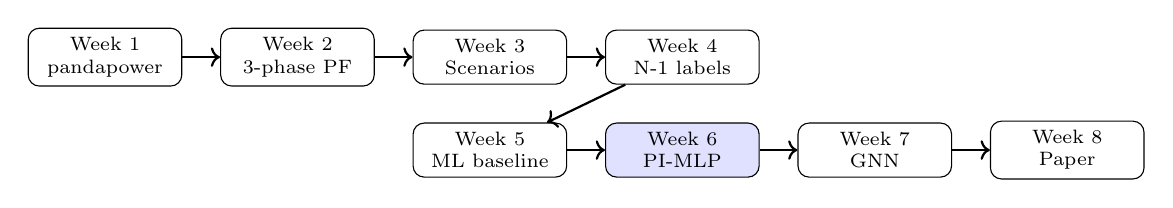
\begin{tikzpicture}[node distance=0.48cm, every node/.style={font=\scriptsize}]
\tikzstyle{box}=[draw, rounded corners, minimum width=1.95cm, minimum height=0.62cm, align=center]
\node[box] (w1) {Week 1\\pandapower};
\node[box, right=of w1] (w2) {Week 2\\3-phase PF};
\node[box, right=of w2] (w3) {Week 3\\Scenarios};
\node[box, right=of w3] (w4) {Week 4\\N-1 labels};
\node[box, below=of w3] (w5) {Week 5\\ML baseline};
\node[box, right=of w5, fill=blue!12] (w6) {Week 6\\PI-MLP};
\node[box, right=of w6] (w7) {Week 7\\GNN};
\node[box, right=of w7] (w8) {Week 8\\Paper};
\draw[->, thick] (w1)--(w2); \draw[->, thick] (w2)--(w3); \draw[->, thick] (w3)--(w4);
\draw[->, thick] (w4)--(w5); \draw[->, thick] (w5)--(w6); \draw[->, thick] (w6)--(w7); \draw[->, thick] (w7)--(w8);
\end{tikzpicture}
\vspace{0.28cm}
\begin{block}{Week 6 的角色}
把 ``会分类'' 的模型升级为 ``知道为什么 unsafe'' 的模型，为 Week 7 图模型和 Week 8 论文消融实验做准备。
\end{block}
\end{frame}

\begin{frame}{从黑箱 ML 到 Physics-informed AI}
\begin{columns}
\begin{column}{0.46\textwidth}
\textbf{Week 5 black-box classifier}
\[
\hat p=f_\theta(x_t,c_k)
\]
\begin{itemize}
  \item 输出 unsafe probability。
  \item 难解释 violation 来源。
  \item ranking 能力不一定稳定。
\end{itemize}
\end{column}
\begin{column}{0.52\textwidth}
\textbf{Week 6 PI-MLP}
\[
(\hat p,\hat s,\hat{\mathbf m})=f_\theta(x_t,c_k)
\]
\begin{itemize}
  \item unsafe probability $\hat p$；
  \item severity $\hat s$；
  \item component margins $\hat{\mathbf m}$；
  \item consistency + ranking losses。
\end{itemize}
\end{column}
\end{columns}
\end{frame}

\begin{frame}{本周的 physics-informed 含义}
\begin{alertblock}{不是}
不是直接把完整三相潮流方程嵌入神经网络，也不是让 MLP 替代 pandapower 的三相潮流求解器。
\end{alertblock}
\begin{block}{而是}
把 Week 4 标签中的物理结构显式加入学习目标：
\begin{itemize}
  \item voltage limits;
  \item phase current / loading limits;
  \item voltage unbalance factor limits;
  \item service-loss / no-slack topology risk;
  \item severity and contingency ranking。
\end{itemize}
\end{block}
\end{frame}

\begin{frame}{部署时刻可用信息与禁止信息}
\begin{columns}
\begin{column}{0.48\textwidth}
\textbf{允许作为输入}
\begin{itemize}
  \item scenario settings;
  \item base-case voltage / VUF / loading;
  \item base-case PCC import;
  \item contingency type;
  \item element metadata。
\end{itemize}
\end{column}
\begin{column}{0.48\textwidth}
\textbf{禁止作为输入}
\begin{itemize}
  \item post-contingency voltage;
  \item post-contingency loading;
  \item post-contingency VUF;
  \item convergence flag;
  \item service loss amount;
  \item violation label / severity。
\end{itemize}
\end{column}
\end{columns}
\vspace{0.15cm}
\[
\mathcal X_{input}\cap \mathcal Y_{post}=\emptyset
\]
\end{frame}

\begin{frame}{Supervised target 设计}
从 Week 4 数据得到：
\[
y\in\{0,1\},\qquad s_{raw}\ge 0
\]
以及 violation flags：
\begin{itemize}
  \item voltage low / voltage high;
  \item loading violation;
  \item VUF violation;
  \item non-convergence;
  \item service loss / critical service loss。
\end{itemize}
Week 6 将这些转成 PI auxiliary targets：
\[
\mathbf m=[m_{V,low},m_{V,high},m_I,m_U,m_S].
\]
\end{frame}

\begin{frame}{Component margin: 低电压}
设低电压阈值为：
\[
V^{min}=0.95\ \mathrm{p.u.}
\]
低电压 margin：
\[
m_{V,low}=\left[\frac{V^{min}-V_{min}^{obs}}{V^{min}}\right]_+
\]
\begin{block}{解释}
当 $V_{min}^{obs}\ge V^{min}$ 时，margin 为 0；当电压越限越严重时，margin 越大。
\end{block}
\end{frame}

\begin{frame}{Component margin: 高电压}
设高电压阈值为：
\[
V^{max}=1.05\ \mathrm{p.u.}
\]
高电压 margin：
\[
m_{V,high}=\left[\frac{V_{max}^{obs}-V^{max}}{V^{max}}\right]_+
\]
\begin{block}{微电网场景}
高 PV、低负荷和反向潮流场景下，高电压 violation 可能成为主导风险。
\end{block}
\end{frame}

\begin{frame}{Component margin: 线路 loading}
线路 loading 阈值：
\[
L^{max}=100\%
\]
loading margin：
\[
m_I=\left[\frac{L_{max}^{obs}}{100}-1\right]_+
\]
\begin{itemize}
  \item $L_{max}^{obs}$ 是 N-1 后最大三相 line loading。
  \item 该目标把 thermal/current risk 显式告诉模型。
\end{itemize}
\end{frame}

\begin{frame}{Component margin: VUF}
VUF 阈值示例：
\[
U^{max}=2\%
\]
VUF margin：
\[
m_U=\left[\frac{U_{max}^{obs}}{U^{max}}-1\right]_+
\]
\begin{alertblock}{三相故事线的核心}
在不平衡微电网中，仅预测 voltage magnitude 不够；VUF 是相不平衡风险的重要标签。
\end{alertblock}
\end{frame}

\begin{frame}{Component margin: service-loss / no-slack}
对于 radial LV feeder，某些 line outage 会导致 downstream load 失供。
\[
m_S=\max(y_{service},y_{critical\ service},y_{no\ slack})
\]
\begin{itemize}
  \item 该目标来自拓扑可供电性逻辑。
  \item 它不依赖连续潮流结果。
  \item 对 PCC outage / no-slack case 尤其重要。
\end{itemize}
\end{frame}

\begin{frame}{PI severity target}
\[
s_{PI}=\max(s_{raw},m_{V,low},m_{V,high},m_I,m_U,m_S)
\]
\begin{block}{目标一致性 proof}
\[
s_{PI}\ge \max_k m_k
\]
这保证 overall severity 不会比任何 component margin 更乐观。
\end{block}
\begin{alertblock}{为什么重要}
如果 severity head 预测很低，但 component head 预测某项越限很大，模型解释会自相矛盾。
\end{alertblock}
\end{frame}

\begin{frame}{模型结构：shared encoder + multi-head}
\centering
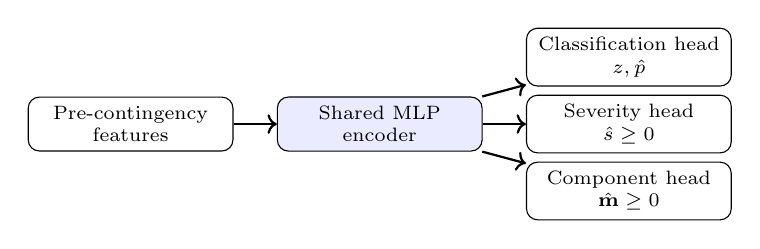
\begin{tikzpicture}[node distance=0.55cm, every node/.style={font=\scriptsize}]
\tikzstyle{box}=[draw, rounded corners, minimum width=2.6cm, minimum height=0.68cm, align=center]
\node[box] (input) {Pre-contingency\\features};
\node[box, right=of input, fill=blue!8] (enc) {Shared MLP\\encoder};
\node[box, right=of enc, yshift=0.85cm] (cls) {Classification head\\$z,\hat p$};
\node[box, right=of enc] (sev) {Severity head\\$\hat s\ge0$};
\node[box, right=of enc, yshift=-0.85cm] (comp) {Component head\\$\hat{\mathbf m}\ge0$};
\draw[->, thick] (input)--(enc); \draw[->, thick] (enc)--(cls); \draw[->, thick] (enc)--(sev); \draw[->, thick] (enc)--(comp);
\end{tikzpicture}
\vspace{0.2cm}
\begin{block}{非负输出}
severity 和 component margins 通过 softplus 输出，避免出现负风险。
\end{block}
\end{frame}

\begin{frame}{Data loss: weighted BCE}
\[
\mathcal L_{cls}= -w_+y\log\hat p-(1-y)\log(1-\hat p)
\]
\begin{itemize}
  \item unsafe/safe 样本可能不平衡。
  \item class weight 只是训练技术，不等于安全保证。
  \item 最终安全性仍要靠 threshold、recall、FNR 和 missed violations 评估。
\end{itemize}
\end{frame}

\begin{frame}{Severity regression loss}
\[
\mathcal L_{sev}=\mathrm{SmoothL1}\left(\log(1+\hat s),\log(1+s_{PI})\right)
\]
\begin{block}{为什么用 $\log(1+s)$}
severity 可能跨不同量级；使用 log transform 可以降低极端样本对训练的支配。
\end{block}
\end{frame}

\begin{frame}{Component margin loss}
\[
\mathcal L_{comp}=\sum_k \mathrm{SmoothL1}\left(\log(1+\hat m_k),\log(1+m_k)\right)
\]
\begin{block}{解释性}
component head 让模型回答：unsafe 是因为 voltage、loading、VUF，还是 service-loss？
\end{block}
\end{frame}

\begin{frame}{Limit consistency loss}
\[
\mathcal L_{cons}=\left[\max_k\hat m_k-\hat s\right]_+^2
\]
\begin{block}{物理含义}
overall predicted severity 至少应覆盖最严重 predicted component violation。
\end{block}
\end{frame}

\begin{frame}{Probability--severity consistency}
如果预测 severity 很大，unsafe probability 不应该很低。
\[
\mathcal L_{prob-sev}=\left(\sigmoid(z)-\sigmoid(\alpha(\hat s-\epsilon))\right)^2
\]
\begin{itemize}
  \item $z$ 是 classification logit。
  \item $\hat s$ 是 predicted severity。
  \item 该项鼓励 probability 和 severity 同向变化。
\end{itemize}
\end{frame}

\begin{frame}{Pairwise ranking loss}
对于一个 mini-batch 中两条样本，如果：
\[
s_i>s_j
\]
希望模型满足：
\[
\hat s_i>\hat s_j
\]
ranking loss：
\[
\mathcal L_{rank}=\left[\delta-(\hat s_i-\hat s_j)\right]_+
\]
\begin{block}{用途}
帮助模型把高风险 contingency 排到 top-k 列表前面。
\end{block}
\end{frame}

\begin{frame}{总损失函数}
\[
\mathcal{L}=\mathcal{L}_{cls}
+\lambda_s\mathcal{L}_{sev}
+\lambda_c\mathcal{L}_{comp}
+\lambda_{cons}\mathcal{L}_{cons}
+\lambda_p\mathcal{L}_{prob-sev}
+\lambda_r\mathcal{L}_{rank}
\]
\begin{alertblock}{课程重点}
每个 loss term 都对应一个工程假设或物理一致性要求；Week 6 不是寻找最优 $\lambda$，而是训练学生建立 loss design 思维。
\end{alertblock}
\end{frame}

\begin{frame}{训练和阈值选择流程}
\centering
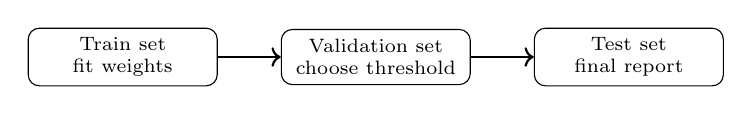
\begin{tikzpicture}[node distance=0.8cm, every node/.style={font=\scriptsize}]
\tikzstyle{box}=[draw, rounded corners, minimum width=2.4cm, minimum height=0.7cm, align=center]
\node[box] (train) {Train set\\fit weights};
\node[box, right=of train] (val) {Validation set\\choose threshold};
\node[box, right=of val] (test) {Test set\\final report};
\draw[->, thick] (train)--(val); \draw[->, thick] (val)--(test);
\end{tikzpicture}
\vspace{0.3cm}
\[
\tau^*=\arg\max_\tau \mathrm{SavedRatio}_{val}(\tau)
\quad \mathrm{s.t.}\quad
\mathrm{Recall}_{val}(\tau)\ge0.95
\]
\end{frame}

\begin{frame}[fragile]{Proof 1: no leakage}
\begin{lstlisting}[language=Python]
leakage_cols = [
    'converged', 'min_vm_pu', 'max_vm_pu',
    'max_vuf_percent', 'max_line_loading_percent',
    'unserved_load_mw', 'violation_label',
    'severity_score', ...]
feature_cols = [c for c in df.columns
                if c not in identifier_cols + leakage_cols]
assert not set(feature_cols).intersection(leakage_cols)
\end{lstlisting}
\begin{block}{结果}
当前数据集通过 no-leakage 检查，输入特征数为 33，one-hot 后维度为 45。
\end{block}
\end{frame}

\begin{frame}{Proof 2: target consistency}
Notebook 检查：
\[
y=0 \Rightarrow s_{raw}=0
\]
\[
y=1 \Rightarrow s_{raw}>0
\]
\[
s_{PI}\ge \max_k m_k
\]
\begin{block}{当前执行}
所有 target consistency checks 通过；validation suite 共 16 项全部通过。
\end{block}
\end{frame}

\begin{frame}{Proof 3: finite loss and gradients}
在一个 mini-batch 上检查：
\begin{itemize}
  \item model output shape 是否正确；
  \item total loss 是否 finite；
  \item 每个可训练参数的 gradient 是否 finite；
  \item predicted probability 是否在 $[0,1]$。
\end{itemize}
\begin{alertblock}{工程意义}
复杂 multi-task loss 很容易因为 log、division、NaN target 导致训练失败，因此必须先做最小 batch proof。
\end{alertblock}
\end{frame}

\begin{frame}{Proof 4: manual confusion matrix}
\[
TP+FP+TN+FN=N_{test}
\]
\[
\mathrm{Recall}=\frac{TP}{TP+FN},\qquad \mathrm{FNR}=\frac{FN}{TP+FN}
\]
\begin{block}{PI-MLP test set 当前结果}
$TP=12, FP=0, TN=8, FN=0$；Recall = 1.00；FNR = 0.00；PF calls saved fraction = 0.40。
\end{block}
\end{frame}

\begin{frame}{Holdout results}
\centering
\begin{tabular}{lrrrrr}
\toprule
Model & Recall & Precision & FNR & Saved & Missed \\
\midrule
BaselineMLP & 1.00 & 0.857 & 0.00 & 0.30 & 0 \\
PI-MLP full & 1.00 & 1.000 & 0.00 & 0.40 & 0 \\
\bottomrule
\end{tabular}
\vspace{0.35cm}
\begin{alertblock}{说明}
当前数据集很小，holdout 结果只用于教学验证；论文版必须扩展 scenario 数量和多随机种子。
\end{alertblock}
\end{frame}

\begin{frame}{Loss ablation results}
\centering
\begin{tabular}{lrrrr}
\toprule
Model & Recall & Precision & Saved & AUPRC \\
\midrule
BaselineMLP & 1.00 & 0.857 & 0.30 & 1.00 \\
PI-MLP no-rank & 1.00 & 0.923 & 0.35 & 1.00 \\
PI-MLP full & 1.00 & 1.000 & 0.40 & 1.00 \\
\bottomrule
\end{tabular}
\vspace{0.3cm}
\begin{block}{教学解读}
本例中 full PI-MLP 在高召回下节省更多 PF 调用；小数据上不宜过度解读绝对数值。
\end{block}
\end{frame}

\begin{frame}[shrink=8]{Training curves}
\centering
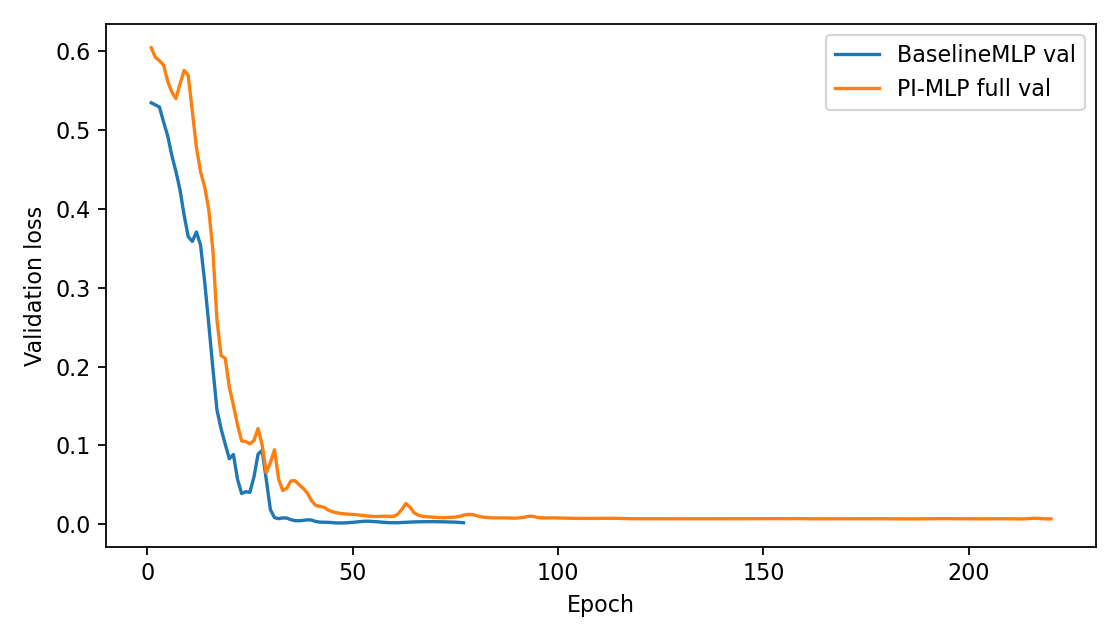
\includegraphics[width=0.82\textwidth]{week6_training_curves.png}
\begin{block}{观察}
validation loss 用于 early stopping；但最终安全指标仍然是 recall、FNR 和 missed violations。
\end{block}
\end{frame}

\begin{frame}[shrink=8]{Precision--recall curves}
\centering
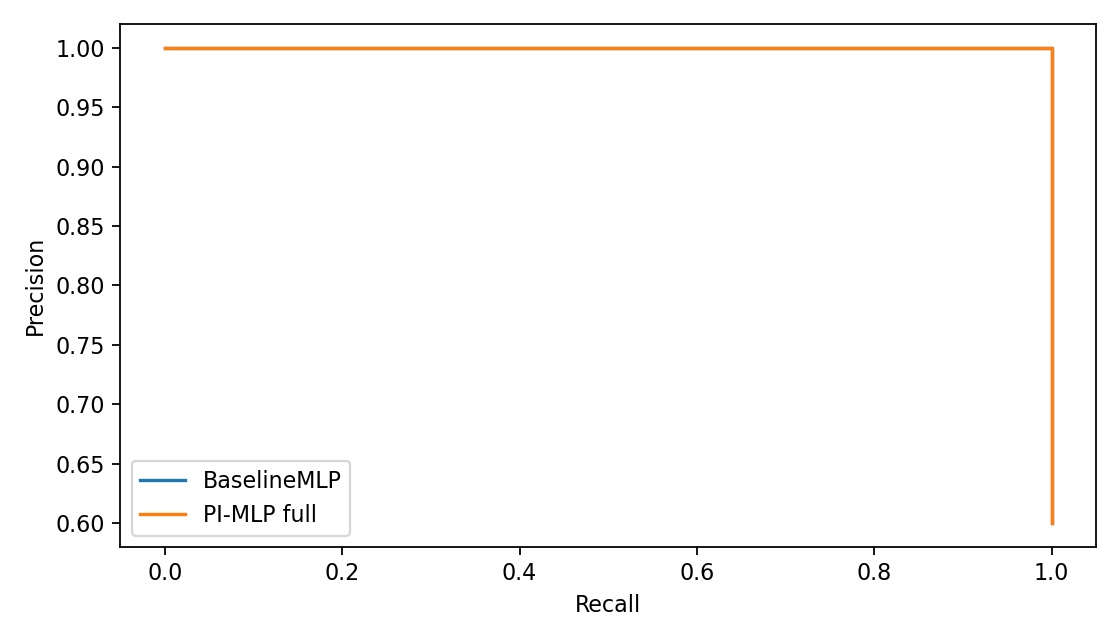
\includegraphics[width=0.78\textwidth]{week6_precision_recall_curves.png}
\begin{block}{为什么看 PR curve}
安全筛查通常是类别不均衡问题，PR curve 比 accuracy 更关注 positive/unsafe 样本识别能力。
\end{block}
\end{frame}

\begin{frame}[shrink=8]{Saved PF calls vs missed violations}
\centering
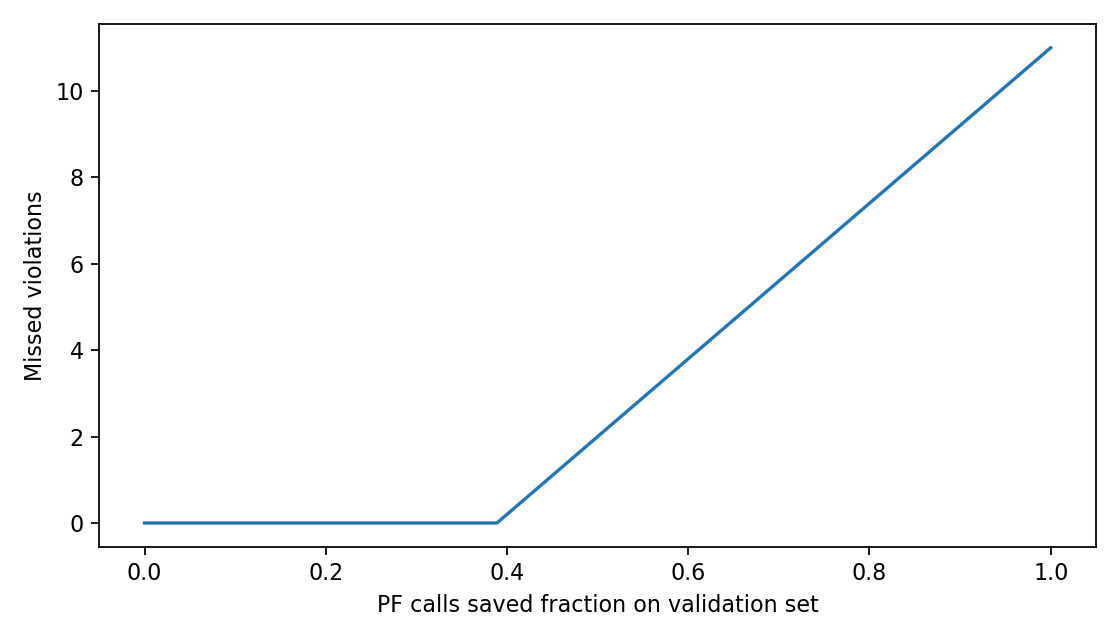
\includegraphics[width=0.78\textwidth]{week6_saved_calls_vs_missed_violations.png}
\begin{block}{工程解释}
任何 saved PF calls 都要和 missed violations 同时报告；不能只说加速。
\end{block}
\end{frame}

\begin{frame}[shrink=8]{True PI severity vs predicted severity}
\centering
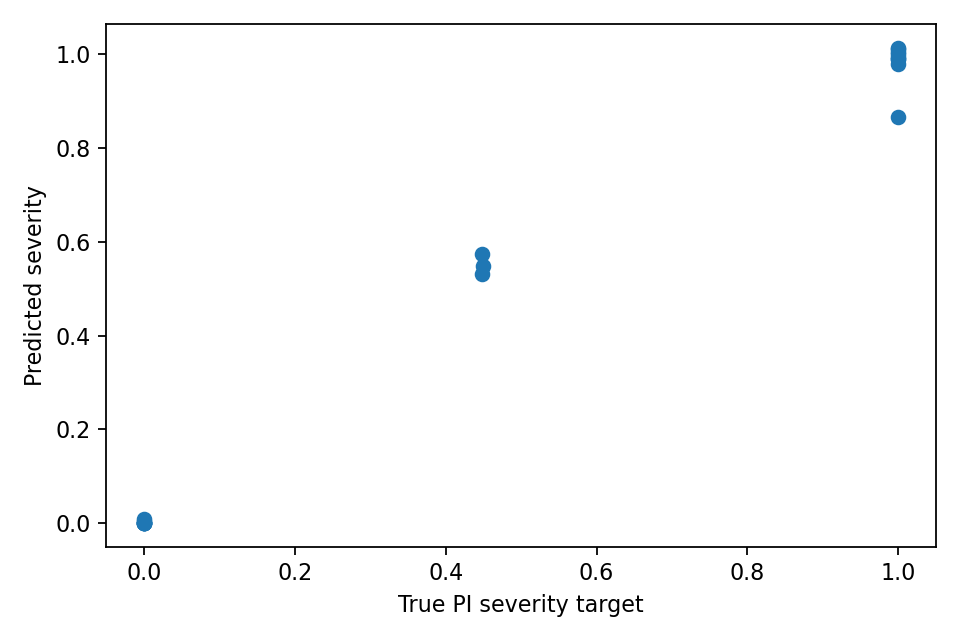
\includegraphics[width=0.68\textwidth]{week6_true_vs_predicted_severity.png}
\begin{block}{用途}
检查 severity head 是否学到风险强弱，而不是只学二元标签。
\end{block}
\end{frame}

\begin{frame}[shrink=8]{Component target distribution}
\centering
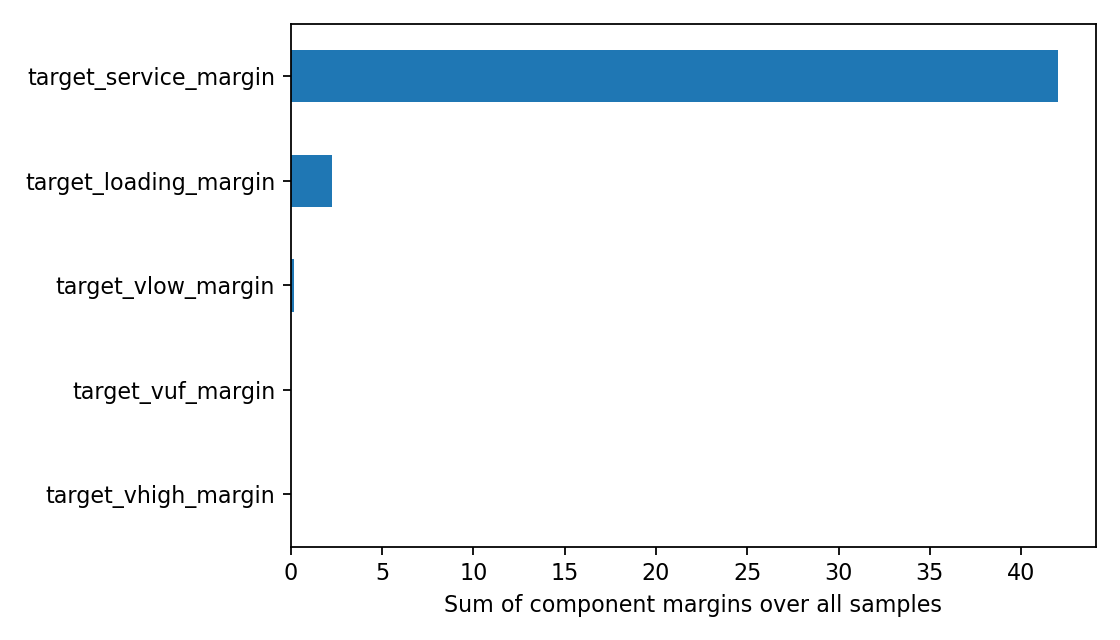
\includegraphics[width=0.78\textwidth]{week6_component_target_distribution.png}
\begin{block}{解释性入口}
component target distribution 能帮助学生理解数据集中主要风险来自哪类约束。
\end{block}
\end{frame}

\begin{frame}{Scenario-group 与 contingency-group CV}
\centering
\begin{tabular}{lrrrr}
\toprule
CV type & Folds & Mean recall & Mean FNR & Mean saved \\
\midrule
Scenario-group & 3 & 0.928 & 0.072 & 0.207 \\
Contingency-group & 3 & 0.760 & 0.240 & 0.413 \\
\bottomrule
\end{tabular}
\vspace{0.35cm}
\begin{alertblock}{关键结论}
contingency-group CV 更难，说明仅靠 tabular metadata 泛化到未见过 contingency 仍有限；这是 Week 7 GNN 的动机。
\end{alertblock}
\end{frame}

\begin{frame}{Reproducibility proof}
Notebook 重新用相同随机种子训练 PI-MLP，并检查 test probabilities：
\[
\max_i |\hat p_i^{(run1)}-\hat p_i^{(run2)}| < 10^{-6}
\]
\begin{block}{当前结果}
最大差异为 $0.000\times 10^0$ 级别，fixed-seed reproducibility check 通过。
\end{block}
\end{frame}

\begin{frame}{Validation suite}
当前 notebook 共检查 16 项：
\begin{itemize}
  \item schema and binary labels;
  \item label/severity consistency;
  \item PI severity dominates component margins;
  \item no-leakage feature set;
  \item disjoint train/validation/test split;
  \item finite preprocessing, finite loss, finite gradients;
  \item manual confusion matrix;
  \item threshold selected from validation;
  \item scenario/contingency group CV disjoint;
  \item fixed-seed reproducibility。
\end{itemize}
\begin{block}{结果}16/16 passed。\end{block}
\end{frame}

\begin{frame}{Week 6 输出文件}
\begin{columns}
\begin{column}{0.52\textwidth}
\textbf{主要 CSV}
\begin{itemize}
  \item training curves;
  \item holdout results;
  \item loss ablation summary;
  \item group CV results;
  \item screening tradeoff;
  \item test predictions;
  \item validation summary。
\end{itemize}
\end{column}
\begin{column}{0.46\textwidth}
\textbf{主要 figures}
\begin{itemize}
  \item training curves;
  \item precision-recall curves;
  \item saved calls vs missed violations;
  \item true vs predicted severity;
  \item component target distribution。
\end{itemize}
\end{column}
\end{columns}
\end{frame}

\begin{frame}{局限性与论文版扩展}
\begin{itemize}
  \item 当前样本数只有 77，用于教学足够，但论文版必须生成更大 scenario pool。
  \item PI-MLP 仍是 tabular model，没有显式编码 feeder topology。
  \item contingency-group CV 暴露出对未见 contingency 的泛化压力。
  \item $\lambda$ 权重尚未系统搜索。
  \item 尚未做 uncertainty calibration / conformal screening。
\end{itemize}
\end{frame}

\begin{frame}{Week 6 到 Week 7 的衔接}
\begin{columns}
\begin{column}{0.48\textwidth}
\textbf{Week 6 PI-MLP}
\begin{itemize}
  \item tabular features;
  \item contingency metadata;
  \item PI loss design;
  \item high-recall screening。
\end{itemize}
\end{column}
\begin{column}{0.48\textwidth}
\textbf{Week 7 Phase-aware GNN}
\begin{itemize}
  \item bus/phase nodes;
  \item line/device edges;
  \item contingency mask;
  \item topology-aware generalization。
\end{itemize}
\end{column}
\end{columns}
\begin{block}{核心动机}把拓扑从 feature engineering 中解放出来，交给图模型显式学习。\end{block}
\end{frame}

\begin{frame}{课堂练习}
\begin{enumerate}
  \item 把 VUF 阈值从 2 percent 改成 1.5 percent，观察 component margin 分布。
  \item 关闭 \texttt{prob\_sev} loss，检查 probability 与 severity 是否仍然同向。
  \item 关闭 ranking loss，对比 top-k contingency ordering。
  \item 把 target recall 从 0.95 改成 1.00，观察 saved PF calls 如何变化。
  \item 思考：哪些内容应该保留到 Week 7 的 GNN loss 中？
\end{enumerate}
\end{frame}

\begin{frame}{参考实现说明}
\begin{itemize}
  \item Notebook 使用 PyTorch 实现 multi-head MLP 和自定义 loss。
  \item 使用 scikit-learn 完成 preprocessing、AUPRC/AUROC 与 GroupKFold。
  \item 所有结果表和图表保存在 \texttt{week6\_outputs\_complete/}。
  \item clean notebook 适合课堂发放；executed notebook 适合教师检查和复现。
\end{itemize}
\end{frame}

\end{document}
